\section{Preamble}
\label{sec:preamble_compound_types}

Before presenting the specifications of the different compound types, let's
define some useful elements of language.

\begin{itemize}
\item \textit{Data borrowing} -- A data borrowing value is a value that points
  to data that is not automatically copied when the value is copied. The
  simplest example of data borrowing is using a pointer type, where the value of
  the pointer provides information about a memory address containing data. The
  data pointed to by the pointer is not copied when the pointer is. An
  illustration of this is presented in Figure~\ref{fig:data_borrowing}.

  \input{images/data_borrowing}

  In the above example, both variable \texttt{x} and \texttt{y} borrow the data
  located in the heap at the address \texttt{0xfa45b987}. By copying the value
  of the variable \texttt{y} into another variable, no copy of the borrowed
  value is made (located on the heap) but only the value directly inside
  \texttt{y} is copied, which s in that case located on the stack. The borrowed
  data can be located on the stack or on the heap, and the same can be said for
  borrowing data. Such memory is called "borrowed" as it can live longer that
  the value pointing to it, and the pointer only borrows its value for reading
  or writing.

  In the case of borrowing data, mutability is crucial because multiple
  variables refer to the same segment of memory. This can lead to unpredictable
  side effects. Memory mutability is employed to manage such behavior and ensure
  that only a few variables have mutable access to values. Most importantly, it
  helps prevent unintentional creation of mutable memory borrowing.

\item \textit{Data movement} -- A data movement is the process of copying a
  value from one segment of memory to another. This can be done through
  assignment, memory copy (or deep copy), function calls, and other operations.
  Data movements are always intended to be explicit, ensuring that no unwanted
  copies are made, which could potentially slow down the program.

\item \textit{lvalue} -- A lvalue refers to the left operand in a \textit{data
  movement} operation. In other words, it is an expression that refers to a
  segment of memory that will be modified as a result of the \textit{data
    movement}. A lvalue can take various forms, including a simple variable, a
  function parameter, an index operation, and more.

\item \textit{rvalue} -- An rvalue is the right operand involved in a
  \textit{data movement} operation. A rvalue can be aliased (using the keyword
  \texttt{alias}), referenced (keyword \texttt{ref}), copied with
  (\texttt{copy}, \texttt{dcopy}), or it can be implicit. Implicit means that
  the \textit{data movement} does not borrow mutable data and can therefore be
  allowed implicitly. In the case of implicit \textit{data movement}, no
  borrowed data is copied and there is no new mutable memory borrowing.

\end{itemize}

\section{Pointers}

Pointers are values storing an address of memory. Pointer types are described
using the \texttt{*} token followed by a type (e.g. \texttt{*i32} describing a
pointer to a \texttt{i32} value). In the beta version of Ymir (compiler written
in c++) the operator \texttt{\&} was used, it was changed as it was also used to
refer to object instances that are in a way pointers but have very different
behavior.

\subsection {Literals}

The \texttt{null} keyword is used to describe a pointer that points to nowhere.
This is the only literal that can be used as pointer value.

\subsection {Construction}

To construct a pointer the unary operator \texttt{\&} can be used on a lvalue (a
variable for example). This operator retreive the address of the value
referenced by the operand, i.e., \texttt{\&a} retreives the address of the
segment of memory referenced by the variable \texttt{a}. By abuse of speech and
simplification, we can say that we retreive the address of the variable
\texttt{a}.

\begin{lstlisting}[style=coloredverbatim]
let a = 12;
let b : *i32 = &a;
\end{lstlisting}

\subsection {Mutability}

Because pointers borrow data from another value (value pointed by the pointer),
their mutability is important. A pointer has two level of mutability:
\begin{enumerate}
\item \texttt{mut *T}, in that case the pointer can be changed but not the value
  inside it.
\item \texttt{mut *(mut T)}, in that case both the value pointed by the pointer
  and the pointer itself are mutable.
\end{enumerate}

A mutable pointer (\textit{level 1}) means that if the pointer is contained
inside another compound type or in a variable its value can be changed. When the
value inside the pointer is created mutability checking is made at compilation
time.

\begin{lstlisting}[style=coloredverbatim]
let dmut a : *i32 = null;

let b = 12;
a = &b; // not allowed 'b' is not mutable
*a = 24; // but it would be modified by this operation


let mut c = 11;
a = &c; // allowed c is mutable
*a = 24; // modify the value of c is allowed
\end{lstlisting}

The keyword \texttt{alias} has to be used on the right operand if data borrowing
is transfered to the left operand. In practice, this means that if the left
operand mutability is of second level (i.e. \texttt{mut *(mut T)}), the keyword
\texttt{alias} has to be used, and right operand must also be of second level
mutability. The keyword can be omitted if the aliasing is obvious (i.e. by
function return, or construction such as the unary operator \texttt{\&}).

\subsection {Properties}

Properties on pointer type can be accessed using the operator ~::~ on a type
expression. The properties are the following:

\vspace{-20pt}%
\begin{center}\begin{adjustbox}{max width=\linewidth}
  \begin{tabular}{|l|ll|}
    \hline
    Name & Meaning & Type\\
    \hline
    \hline
    \texttt{init} & The initial value \texttt{null} & \texttt{typeof(x)}\\
    \texttt{inner} & The inner type contained in the pointer type & None\\
    & This property returns a type expression, not a value &\\
    \hline
    \texttt{typeid} & A string encoding the name of the type & \texttt{[c8]} \\
    \hline
  \end{tabular}
\end{adjustbox}\end{center}

\subsection {Casting}

A pointer type can be casted using the cast operator \texttt{cast!T(V)}, into
any pointer type. Pointer is a really low level type with just few guarantees,
but some operations rely on that possibility to perform generic operations
(common traits, \texttt{Packable} for example). Mutability of the result is the
same as the mutability of the operand. This is the only allowed casts on pointer
types.

\subsection {Unary operators}

The unary operator \texttt{*} is used on a pointer value to dereference it and
access the value pointed by the pointer. This operation is unsafe, and might
throw a \texttt{SegFault} exception. If the operation does not throw anything it
does not necessarily mean that the pointer was correctly created. Because this
operation is unsafe, and can only be used in an \texttt{unsafe} context.

\begin{lstlisting}[style=coloredverbatim]
let i = 10;
let x = &i;

unsafe {
  let j = *x;
}
\end{lstlisting}

\subsection {Binary operators}

Binary operators are divided into 3 groups:
\begin{itemize}
\item Math: Pointer arithmetic is allowed using a \texttt{usize} as right
  operand. Unlike in C language, the arithmetic does not depend on the size of
  the data pointed by the pointer. The operation adds a number of bytes to the
  address, meaning that the addition operation using a left operand whose value
  is \texttt{0xabc0} and a right operand \texttt{8us} will always have the value
  \texttt{0xabc8} no matter the type of content pointed by the pointer. The
  behavior is not the same with index operator. The type of the result of the
  operation always takes the same type as the left operand.

  %%
  \vspace{-20pt}%
  \begin{center}\begin{adjustbox}{max width=1\linewidth}
    \begin{tabular}{|c|lll|}
      \hline
      Operator & Operation & Commutative & Example \\
      \hline
      \hline
      \texttt{+} & Addition & Yes & \texttt{\&a + 2us} \\
      \texttt{-} & Substraction & No & \texttt{\&a - 2us} \\
      \hline
    \end{tabular}
  \end{adjustbox}\end{center}

\item Logical: Comparison operators always return a value of type \texttt{bool}
  and are only usable when the two operands are of the same pointer type (e.g.
  \texttt{*i32} with \texttt{*i32}).

  \vspace{-15pt}%
  \begin{center}\begin{adjustbox}{max width=1\linewidth}
    \begin{tabular}{|c|lll|}
      \hline
      Operator & Operation & Commutative & Example \\
      \hline
      \hline
      \texttt{is} & Equality test & Yes & \texttt{\&a is \&a == true}\\
      \texttt{!is} & Equality test & Yes & \texttt{\&a !is \&a == false}\\
      \texttt{<} & Lower than & No & \texttt{\&a < \&a + 1us == false}\\
      \texttt{>} & Greater than & No & \texttt{\&a > \&a - 1us == false}\\
      \hline
    \end{tabular}
  \end{adjustbox}\end{center}

\item Affectation: The affectation operator are usable when the two operands
  have strictly the same pointer type. The mutability level of the left operand
  must be lower than or equal to the mutability level of the right operand.
  Affectation operators can be mixed with math operators (e.g. \texttt{+=},
  \texttt{-=}). In that case the operation is rewritten into \texttt{x = x + y}
  and \texttt{y} must be a value of type \texttt{usize}.

  \begin{lstlisting}[style=coloredverbatim]
let mut a = 11;
let dmut b = &a;

let mut c = &a;
b = c; // not allowed it will discard the const property
c = b; // No problem the mutability level of c is lower than the one of b

c += 1us;

let dmut d = &a;
b = alias d; // alias is needed, data is borrowed
  \end{lstlisting}

\end{itemize}

\subsection {Index operator}

The index operator can be used on a pointer left operand using an int value as
an index right operand. The result of the operation is the dereferencement of
the pointer value with the offset of the value used as index. Unlike pointer
arithmetic using the \texttt{+} and \texttt{-} operator, the index operator
takes into account the size of the data pointed by the pointer, meaning that the
index operation \texttt{(\&a)[7]} is strictly transformed into \texttt{*(\&a +
  (7us * sizeof (typeof(\&a)::inner)))}. This operation is unsafe, as it
dereference a raw pointer.

\smallskip

\begin{lstlisting}[style=coloredverbatim]
let mut a = 12;
let dmut b = &a;

unsafe {
  b [0] = 89;
}
assert (a == 89);
\end{lstlisting}

\smallskip
The result value mutability depends on the level of mutability of the pointer
operand. If the pointer operand mutability level is 2, then the result can be
used as a lvalue.

\section {Tuples}


Tuple are anonymus structure storing a set of data of different types. They are
described as a list of types enclosed within parentheses (e.g. \texttt{(i32,
  f32, c8)}). A tuple can have only one inner type, in that case the token
\texttt{,} is added after the definition of the inner type (e.g.
\texttt{(i32,)}).

\subsection {Literals}

Tuple literals are described as a list of values enclosed by parentheses tokens,
for example \texttt{(1, 'r', false)} is a tuple literal whose type is
\texttt{(i32, c32, bool)}. Tuple containing only one value must contain the
token \texttt{,} after the declaration of the value, in order to distinguish
them from priority operation enclosed within parentheses.

\begin{lstlisting}[style=coloredverbatim]
let a = (1, 'r', false);
let b : (i32,) = (23,); // tuple value
let c : i32 = (23); // int value
\end{lstlisting}

\noindent Tuple inner values are constructed in the order they are written. In the
following example, the function \texttt{foo} is called before the function
\texttt{bar}.

\begin{lstlisting}[style=coloredverbatim]
def foo ()-> i32 {
  println ("In foo.");
  12
}

def bar ()-> f32 {
  println ("In bar.");
  34.0f
}

let a = (foo (), bar ());
\end{lstlisting}

\subsection {Mutability}
\label{sec:tuple_mutability}

The mutability of tuple values cannot be described as a mutability level as it
could be for other compound types. In the case of tuple, the mutability is
defined as a tree, where each node of the tree depend on the mutability of its
parent. For example, the mutability of the following tuple type \texttt{mut (mut
  i32, f32, dmut *c8)} is presented in the Figure~\ref{fig:tuple_mutability}.

\begin{center}
  \scalebox{1.3}{
    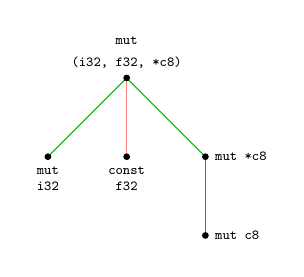
\begin{tikzpicture}

      \draw[-, black!30!green] (0,0) -- (-1,-1);
      \draw[-, red!50] (0,0) -- (0,-1);
      \draw[-, black!30!green] (0,0) -- (1,-1);
      \draw[-, black!30!green] (1,-1) -- (1,-2);

      \filldraw (0, 0.3) node[align=center, above] {\texttt{\tiny{mut}}};
      \filldraw (0, 0) circle (1pt) node[align=center, above] {\texttt{\tiny{(i32, f32, *c8)}}};
      \filldraw (-1,-1) circle (1pt) node[align=center, below]{\texttt{\tiny{mut}}};
      \filldraw (-1,-1.2) node[align=center, below]{\texttt{\tiny{i32}}};
      \filldraw (0,-1) circle (1pt) node[align=center, below]{\texttt{\tiny{const}}};
      \filldraw (0,-1.2) node[align=center, below]{\texttt{\tiny{f32}}};
      \filldraw (1,-1) circle (1pt) node[align=center, right]{\texttt{\tiny{mut *c8}}};
      \filldraw (1,-2) circle (1pt) node[align=center, right]{\texttt{\tiny{mut c8}}};


    \end{tikzpicture}
  }
  \captionof{figure}{\label{fig:tuple_mutability} Example of tuple mutability}
\end{center}


Mutability level of inner types is important only when they borrow data. In the
previous example presented in Figure~\ref{fig:tuple_mutability}, only the
mutability of the inner type \texttt{*c8} is important during data movement. In
other word a value of type \texttt{mut (i32, f32, dmut *c8)} can be passed to it
without any problem. As for any borrowing type, the keyword \texttt{alias} has
to be used when data is borrowed.

\begin{lstlisting}[style=coloredverbatim]
let mut x = 't'c8;
let mut a : mut (mut i32, f32, dmut *c8) = (1, 12.0f, &x);
let mut b : mut (i32, f32, dmut *c8) = (1, 7.0f, null);

a = alias b; // no problem
b = alias a; // no problem either

let c : (i32, f32, *c8) = (1, 7.0f, &x);
a = alias c; // not allowed, it would dicard constant property of the third field
\end{lstlisting}

Tuple types having mutable values that are not borrowing data are considered non
borrowing types, and therefore don't need \texttt{alias} during data movement.
In practice all the data of this kind of tuples are copied during data movement.

\subsection {Properties}

Properties on pointer type can be accessed using the operator \texttt{::} on a
type expression. The properties are the following:
\smallskip

\begin{center}
  \begin{adjustbox}{max width=\linewidth}
    \begin{tabular}{|l|ll|}
      \hline
      Name & Meaning & Type\\
      \hline
      \hline
      \texttt{init} & The inital value of the tuple & \texttt{usize} \\
      & where every inner field are set to \texttt{T::init} & \\
      \Xhline{0.001pt}
      \texttt{arity} & The number of inner elements of the tuple type & \texttt{usize}\\
      \hline
      \texttt{init} & A string encoding the name of the type & \texttt{[c8]} \\
      \hline
    \end{tabular}
  \end{adjustbox}
\end{center}

\smallskip

Inner types are not accessible through the operator \texttt{::}, but are
accessible using \texttt{\_\_pragma}. Pragma are presented in
Section~\ref{sec:pragmas}.

\subsection {Binary operators}

Binary operators are divided into 3 groups:
\begin{itemize}
\item Access: The operator \texttt{.} is used to access to a given field of the
  tuple. The right operand must be of an int type and be within the range of
  \texttt{0} and the arity of the tuple being accessed. The result of the
  operation takes the type of the field at the index described by the right
  operand, and so is the value. The first field index is \texttt{0}.

  \begin{lstlisting}[style=coloredverbatim, linewidth=0.95\linewidth]
let mut a : (mut i32, f32) = (8, 8.f);

a._0 = 7; // allowed first field is mutable
a._1 = 1.f; // not allowed, second field is not mutable

let c = a.(12 - 11); // accessing the field at index 1
  \end{lstlisting}

\item Comparison: The comparison operators \texttt{==} and \texttt{!=} are
  defined on tuples when each of the inner types are comparable. It compares all
  the fields of two tuples, and checks wether all the inner values are equals
  for \texttt{==}, or at least one inner value is different between the two
  operands for the operator \texttt{!=}.

  There is no order relation between tuples, even if they have the same type as
  in general such comparison would be senseless.

\item Affectation: Affectation operator creates a \textit{data movement} from
  the right operand to the left operand. Mutability has to be respected when
  data is borrowed. Data mutability on tuples was already presented in
  Section~\ref{sec:tuple_mutability}.

\end{itemize}

\subsection {Dollar operator}

The dollar operator is usable within an Access binary operation in the right
operand expression. The dollar value takes the value of the arity of the tuple,
and its type is \texttt{usize}. Its value is known at compilation time.

\begin{lstlisting}[style=coloredverbatim]
let a = (1, 9.0f, 'r');

let b = a.($ - 1us); // access the last value, i.e. 'r'
\end{lstlisting}

\subsection {Tuple expansion}

Tuples have a specific operator named \texttt{expand} that transform them into a
list of parameters. The expansion of tuple is useful to create other tuples, or
passing the data of the tuple as function parameters.

\begin{lstlisting}[style=coloredverbatim]
def foo (a : i32, b : f32) {}

let a = (1, 5.f);

 // transform a into a list of values
let b : (i32, f32, c32) = (expand a, 't');

foo (expand a); // transform a into a list of parameters
\end{lstlisting}

Such operation is made at compilation time, and is simply a rewritte operation
that is less verbose. Indeed, in the previous example, the line \texttt{foo
  (expand a)}, is rewritten into \texttt{foo (a.0, a.1)}. The mutability level
of the expanded values is always \texttt{1} meaning tuple expansion can never
borrow mutable data. Tuple expansion are usefull in variadic template functions,
to write generic operations on a list of variadic parameters.

\subsection {Tuple deconstruction}

Tuple can be used to declare multiple variable at once, using the same
\texttt{let} declaration. We call this declaration a tuple deconstruction, as it
splits the values of the tuple into a list of variables.

\begin{lstlisting}[style=coloredverbatim]
  // a is mutable, but not b nor c
let (mut a, b, c) = (1, 't', 12.f);

assert (a == 1 && b == 't' && c == 12.f);
\end{lstlisting}

A variadic variable can be used as the last variable declaration in such
deconstruction with the token \texttt{...}. In that case it's type is always a
tuple that takes all the values in the tuple that are left, and are not
associated with other variables.

\begin{lstlisting}[style=coloredverbatim]
let (a, b...) = (1, 2, 3);

assert (a == 1);
assert (b == (2, 3));
\end{lstlisting}

The mutability level of variables declared using tuple deconstruction can be
mutable by using the keywords \texttt{mut} or \texttt{dmut} on specific
variables of the tuple deconstruction (i.e. \texttt{let (dmut a, b) = alias
  t;}). In that case the right operand must match the mutability, and be aliased
explicitly.

\subsection {Tuple iteration}

Tuples are iterable types, thus they can be used as the iterable value of a
\texttt{for} loop. In practice because such iteration would create iterator
variables with different types, the iteration is unrolled at compilation time.
The tuple value is constructed only one time before entering any loop body.

\begin{lstlisting}[style=coloredverbatim]
let a = (1, 't', 89.0f);
for i in a {
    println (i);
}

// would be rewritten into
println (a._0);
println (a._1);
println (a._2);
\end{lstlisting}

Two variables are usable as iterators, the first one being the index of the
iteration, and the second one being the value inside the tuple. If only one
variable is defined, only the value of the tuple fields is contained in the
iterator. Iterators are always immutable and never used as references, however
this limitation can be easily couterfeited, using the index iterator to access
the tuple.

\begin{lstlisting}[style=coloredverbatim]
let dmut a = (1, 2, 3);
for i, _ in a {
    a.(i) = 9;
}

assert (a == (9, 9, 9));
\end{lstlisting}

More information about \texttt{for} loops is presented in
Section~\ref{sec:for_loops}.

\section {Ranges}

Range is a compound type composed of four elements describing a range of values.
The four elements are the following: \texttt{fst} the first value of the range
(e.g. \texttt{0}), \texttt{scd} the final value of the range (e.g. \texttt{10}),
\texttt{step} the step of the range (e.g. \texttt{2}), and \texttt{contains} of
type bool specifiying wether the final value \texttt{scd} is included in the
range or not. There are only three kinds of types that can be describing the
inner components of a range: integer, floating point and character types. Range
type is defined using the inner type followed by the token \texttt{..} (e.g.
\texttt{i32..} describes a range of \texttt{i32} values).

Range are useful for iteration, or accessing a subset of values (for example a
subset of a slice).

\subsection {Literals}

Range literals are described using the token \texttt{..} or the token
\texttt{...}. The token \texttt{..} is used to define a range whose final value
is not included in the range, when the \texttt{...} token defined a range whose
final value is included. If different tokens are used to describe the literal,
the type is the same, and the token \texttt{..} is always the only token used to
describe a range type.

\begin{lstlisting}[style=coloredverbatim]
let a : i32.. = 0 .. 2;
let b : i32.. = 0 ... 2;

assert (a.fst == b.fst);
assert (a.scd == b.scd);
assert (a.step == b.step);
assert (!a.contains && b.contains);
\end{lstlisting}

Range values can be decreasing, in that case the step is negative. One can note
that for ranges of unsigned integers and character values, a negative value for
the step is in theory impossible to have. However, there is some cheating
happening here using the limitation of overflowing of the types to create a
value that when added to \texttt{fst} equals to \texttt{fst - abs (step)} (in
practice this is exactly the same as adding a negative value at the binary
level, but it is not really the valid high level representation). For that
reason one can consider that step is always a signed version of the type even if
the field type is considered to be the same as the type of the inner values
(\texttt{fst} and \texttt{scd}) and thus that one bit of its encoding is always
used for the sign.

The \texttt{fst} value of range literal is constructed before the \texttt{scd}
value. In the following example, the function \texttt{foo} is called before the
function \texttt{bar}.

\begin{lstlisting}[style=coloredverbatim]
def foo ()-> i32 {
  println ("In foo.");
  12
}

def bar ()-> i32 {
  println ("In bar.");
  1
}

let a = (foo ()) .. (bar ());
\end{lstlisting}

\subsection {Mutability}

As one might expect range values don't borrow any data, and every field
contained in the value is copied during data movement, thus there is no need to
worry about mutability making the type not aliasable. A mutable range can modify
its inner fields. Even if the range type is a compound type, it behaves exactly
as a scalar type as it can never contain any borrowed data.

\subsection {Properties}

Properties on range type can be accessed using the operator \texttt{::} on a
type expression. The properties are the following:

\begin{center}\begin{adjustbox}{max width=\linewidth}
  \begin{tabular}{|l|ll|}
    \hline
    Name & Meaning & Type\\
    \hline
    \hline
    \texttt{init} & The initial value ranging from \texttt{T::init} & \texttt{typeof (x)}\\
    & to \texttt{T::init} with a step of \texttt{T::init} and & \\
    & with contains set to \texttt{false} where \texttt{T} is & \\
    & the inner type (e.g. \texttt{i32} for \texttt{i32..}). &\\
    \Xhline{0.001pt}
    \texttt{inner} & The inner type contained in the range type & None \\
    & This property returns a type expression, not a value & \\
    \hline
    \texttt{typeid} & A string encoding the name of the type & \texttt{[c8]} \\
    \hline
  \end{tabular}
\end{adjustbox}\end{center}


\subsection {Binary operators}

Binary operators are divided into 4 groups:

\begin{itemize}
\item Access: The operator \texttt{.} is used to access to the field of the
  range type. The right operand being the name of the field to access. These
  fields are described in the following table.

  \vspace{-20pt}%
  \begin{center}\begin{adjustbox}{max width=\linewidth}
    \begin{threeparttable}
      \begin{tabular}{|l|ll|}
        \hline
        Name & Value & Type\\
        \hline
        \hline
        \texttt {fst} & The first value of the range & \texttt{typeof (x)::inner} \\
        \texttt {scd} & The second value of the range & \texttt{typeof (x)::inner} \\
        \texttt {step} & The step of the range & \textit{T}$^{1^{\phantom{j}}}$ \\
        \texttt {contains} & The field describing wether or  & \texttt{bool} \\
        & not the scd value is contained in the range &\\
        \hline
      \end{tabular}
      \begin{tablenotes}
      \item[1.]\small \textit{signed version of the inner type for ranges on int
        type, and a int type for ranges on characters types, and
        \texttt{typeof(x)::inner} for ranges on float types}
      \end{tablenotes}
    \end{threeparttable}
\end{adjustbox}\end{center}

Accessed fields are mutable if and only if the range is mutable.

\item Contains: The operator \texttt{in} and \texttt{!in} are used to check
  wether a value is contained inside a range value. In that case the type of the
  left operand must be the same as the inner type of the right operand, and the
  type of the right operand must be a range type.

\item Comparison: Range are comparable using the operators \texttt{==} and
  \texttt{!=}, checking the equality (or inequality) of every field of the
  range. The left and right operand must have exactly the same type.

\item Affectation: A range value can be a lvalue if and only if it is mutable.
  \begin{lstlisting}[style=coloredverbatim]
let mut a = 0 .. 7;

a = 7 .. 1;
  \end{lstlisting}

\end{itemize}

\subsection {Range iteration}

Ranges are iterable types, therefore they can be used as the iterable value of a
\texttt{for} loop. Only one imutable variable can be declared when iterating
over a range value. This iterator variable takes the value of the \texttt{fst}
field of the range, and increment by the \texttt{step} field until it reaches
the \texttt{scd} field. If the range is a containing range (i.e.
\texttt{contains} field is true), then the \texttt{scd} field is included in the
iteration.

\begin{lstlisting}[style=coloredverbatim]
for i in 0 .. 7 {
    print (i, ' '); // 0 1 2 3 4 5 6
}

for i in 0 ... 7 {
    print (i, ' '); // 0 1 2 3 4 5 6 7
}

for i in 7 .. 0 {
    print (i, ' '); // 7 6 5 4 3 2 1
}
\end{lstlisting}

More information about \texttt{for} loops is presented in
Section~\ref{sec:for_loop}.

\section{Arrays}

An array is a compound type containing a list of values of the same type stored
in continuous memory segment and whose size is known at compilation time. An
array type is described using the following syntax \texttt{[T ; N]} where
\texttt{T} is the inner type of the array, and \texttt{N} is an integer value
describing the number of elements contained in the array.

\subsection {Literals}

Array literals are a list of values enclosed within brackets \texttt{[} and
  \texttt{]}. An array literal of size \texttt{0} contains no data, and is just
the brackets. Array literal are indistinguishable from slice literals (cf.
Section~\ref{sec:slices}), it is the type of lvalue operand that define wether
to create a slice or an array value. By default, if the type of the lvalue is
not defined the operand type is always a slice type.

\begin{lstlisting}[style=coloredverbatim]
def foo (x : [i32 ; 4]) {// ...}

let a = [1, 2, 3]; // slice [i32]
let b : [i32 ; 3] = [1, 2, 3]; // array [i32 ; 3]


foo ([1, 2, 3, 4]); // calling with an array [i32 ; 4]
\end{lstlisting}

Array literals can also be defined using the array construction syntax. The
syntax is close to the type description of the array type, but using a value
instead of a type \texttt{[V ; N]}. Each element of the array will take the
value \texttt{V}.

\begin{lstlisting}[style=coloredverbatim]
let a = [12 ; 2]; // an array of i32 of size 2, where every element is equal to 12

assert (a [0] == 12 && a [1] == 12);
\end{lstlisting}

Array inner values are constructed in the order they are written. In the
following example, the function \texttt{foo} is called before the function
\texttt{bar}.

\begin{lstlisting}[style=coloredverbatim]
def foo ()-> i32 {
  println ("In foo.");
  1
}

def bar ()-> i32 {
  println ("In bar.");
  2
}

let a : [i32 ; 2] = [foo (), bar ()];
\end{lstlisting}

\subsection {Mutability}

Arrays don't borrow data on their own, as they are in fact the data of the
arrays themselves. Meaning that during data movement all the datas contained in
an array are copied. As for tuples, mutability level of array is therefore only
important if the inner type of the array is a type that borrows data. Memory
representation of the following example is presented in
Figure~\ref{fig:data_repr_array}.

\begin{lstlisting}[style=coloredverbatim]
let dmut a : [i32 ; 3] = [1, 2, 3];

let dmut b = a; // no need for alias
                // a and b don't refer to the same memory segment

let i = 89;
let c : [*i32 ; 1] = [&i];

let dmut d = c; // not allowed, discard const property of the inner type
\end{lstlisting}

\begin{figure}[H]
  \centering
  \scalebox{0.7}{
    \begin{tikzpicture}
      % ================ Axis ========================
      \draw (0, 0) -- coordinate (LEFT) (0, 0);
      \draw[->](0, 10) -- coordinate (YAx) (0, 0);
      \draw[->](7.2, 10) -- coordinate (YAx) (7.2, 0);
      \draw[Box] (3.5, 10.7) -- (3.5, 10.7) node[anchor=center]{\textbf{STACK}};

      \filldraw (0, 8) circle (1pt) node[align=center, left] {+0};
      \filldraw (0, 7.3) circle (1pt) node[align=center, left] {+4};
      \filldraw (0, 6.5) circle (1pt) node[align=center, left] {+8};
      \filldraw (0, 5.8) circle (1pt) node[align=center, left] {+12};
      \filldraw (0, 5.1) circle (1pt) node[align=center, left] {+16};
      \filldraw (0, 4.4) circle (1pt) node[align=center, left] {+20};
      \filldraw (0, 3.7) circle (1pt) node[align=center, left] {+24};
      \filldraw (0, 3) circle (1pt) node[align=center, left] {+28};
      \filldraw (0, 2.3) circle (1pt) node[align=center, left] {+32};
      \filldraw (0, 1.6) circle (1pt) node[align=center, left] {+36};
      \filldraw (0, 1) circle (1pt) node[align=center, left] {+40};

      %% % ================ Foo ========================
      \fill[black!10] (0.2, 10) rectangle (7, 9.5);
      \draw[Box] (3.5, 9.2) -- (3.5, 9.2) node[anchor=center]{\textbf{.}};
      \draw[Box] (3.5, 9) -- (3.5, 9) node[anchor=center]{\textbf{.}};
      \draw[Box] (3.5, 8.8) -- (3.5, 8.8) node[anchor=center]{\textbf{.}};

      \draw[line width=1pt] (0.18, 8.5) rectangle (7.02, 0.95);
      \fill[olive!10] (0.2, 8) rectangle (7, 0.95);
      \draw[Box] (3.5, 8.2) -- (3.5, 8.2) node[anchor=center]{\emph{foo}};

      \draw[Box] (0.5, 6.95) -- (0.5, 6.95) node[anchor=center]{\textbf{\textit{a}}};
      \draw[line width=0.005pt] (0.3, 7.95) rectangle (6.8, 5.95);

      \draw[Box] (3.5, 7.65) -- (3.5, 7.65) node[anchor=center]{$1$};
      \draw[Box] (3.5, 6.95) -- (3.5, 6.95) node[anchor=center]{$2$};
      \draw[Box] (3.5, 6.25) -- (3.5, 6.25) node[anchor=center]{$3$};

      \draw[Box] (0.5, 4.85) -- (0.5, 4.85) node[anchor=center]{\textbf{\textit{b}}};
      \draw[line width=0.005pt] (0.3, 5.75) rectangle (6.8, 3.85);

      \draw[Box] (3.5, 5.5) -- (3.5, 5.5) node[anchor=center]{$1$};
      \draw[Box] (3.5, 4.8) -- (3.5, 4.8) node[anchor=center]{$2$};
      \draw[Box] (3.5, 4.1) -- (3.5, 4.1) node[anchor=center]{$3$};

      \draw[Box] (0.5, 3.4) -- (0.5, 3.4) node[anchor=center]{\textbf{\textit{i}}};
      \draw[line width=0.005pt] (0.3, 3.65) rectangle (6.8, 3.15);
      \draw[Box] (3.5, 3.4) -- (3.5, 3.4) node[anchor=center]{$89$};

      \draw[Box] (3.5, 2.7) -- (3.5, 2.7) node[anchor=center]{-};

      \draw[Box] (0.5, 1.6) -- (0.5, 1.6) node[anchor=center]{\textbf{\textit{c}}};
      \draw[line width=0.005pt] (0.3, 2.35) rectangle (6.8, 1.05);
      \draw[Box] (3.5, 1.6) -- (3.5, 1.6) node[anchor=center]{\emph{ptr~=}~$foo+24$};

      \draw[-Stealth, thick, shorten >=0.2pt] (7.3, 1.6) to [out=-10,in=20, bend right=45] node[below left, yshift=1mm] {} (7.3, 3.4);

    \end{tikzpicture}
  }
  \caption{\label{fig:data_repr_array} Example of memory representation of array values}
\end{figure}


\subsection {Properties}

Properties on array type can be access using the operator ~::~ on a type
expression. The properties are the following:

\vspace{-20pt}%
\begin{center}\begin{adjustbox}{max width=\linewidth}
  \begin{tabular}{|l|ll|}
    \hline
    Name & Meaning & Type\\
    \hline
    \hline
    \texttt{init} & The initial value, where all & \texttt{typeof(x)} \\
    & inner values are set to  & \\
    \Xhline{0.001pt}
    \texttt{size} & The static size of the array (is equal to \texttt{.len}) & \texttt{usize} \\
    \Xhline{0.001pt}
    \texttt{inner} & The inner type contained in the pointer type & None\\
    & This property returns a type expression, not a value &\\
    \hline
    \texttt{typeid} & A string encoding the name of the type & \texttt{[c8]} \\
    \hline
  \end{tabular}
\end{adjustbox}\end{center}

\subsection {Binary operators}

Binary operators are divided into four groups:

\begin{itemize}
\item Access: The operator \texttt{.} is used to access to fields describing the
  array type. The right operand is the name of the field to access. These fields
  are described in the following table.
  \vspace{-20pt}%
\begin{center}\begin{adjustbox}{max width=\linewidth}
  \begin{tabular}{|l|ll|}
    \hline
    Name & Value & Type\\
    \hline
    \hline
    \texttt{len} & The size of the array & \texttt{usize} \\
    \texttt{ptr} & The pointer to the first element  & \texttt{*(typeof (x)::inner)} \\
    & of the array & \\
    \hline
  \end{tabular}
\end{adjustbox}\end{center}

  The \texttt{len} field is known at compilation time, and therefore usable in a
  \texttt{cte} expression. The type of the \texttt{ptr} field has the same
  mutability level as the array type. As one can note, array does not really
  have fields. The values are constructed from the array information,
  \texttt{ptr} takes the address of the array as value, and \texttt{len} is an
  integer literal containing the length of the array in number of contained
  elements.

\item Concatenation: Concatenation operator \texttt{\~} is used to create an
  array or a slice containing the values of two arrays or slices. The operator
  is usable when the left and right operand have the same inner type, no matter
  their relative sizes. The mutability of the generated value is the strictest
  mutability between the two operands. For example, the type and mutability of
  \texttt{([*i32 ; 4]) \~\ (dmut [*i32 ; 2])} is \texttt{[*i32 ; 6]} to avoid
  discarding constant property of the values containined in the left operand. As
  one can note the type of the generated value is an array type whose size is
  the sum of the size of the left and right operands.

  The operator is also usable when one of the two operands is a slice. In that
  case the return value of the operation will therefore be a slice instead of an
  array as its size cannot be known at compilation time. This operation is in
  fact carried out by the slice operand more than by the array operands, and
  will be further discuss in Section~\ref{sec:slices}.

  The operator \texttt{\~} was selected to avoid confusion with the \texttt{+}
  that would have different behavior depending on the operands. Concatenation is
  not really a math operation, as \texttt{+} would preferably refer to an
  addition of all the inner values of two arrays, more than to their
  concatenation.

  Concatenation operator is obviously not commutative.

  \begin{lstlisting}[style=coloredverbatim]
let a : [i32 ; 3] = [1, 2, 3];
let b : [i32 ; 2] = [4, 5];

let c : [i32 ; 5] = a ~ b;

assert (c == [1, 2, 3, 4, 5]);
  \end{lstlisting}

\item Comparison: Binary comparison operators are usable using two arrays with
  the same inner type, or one array and one slice with the same inner type. The
  result of the operation always takes the type \texttt{bool}. For the operators
  to work, the inner type of the array must also define the comparison
  operators. Lexical order is used therefore the size of an array is only used
  when one of the two operands is a prefix to the other (e.g. \texttt{[1, 2]} is
  a prefix of \texttt{[1, 2, 3]}, therefore \texttt{[1, 2, 3]} is considered
  greater than \texttt{[1, 2]}, however \texttt{[1, 3]} is greater than
  \texttt{[1, 2, 3]}).

  \vspace{-20pt}%
  \begin{center}\begin{adjustbox}{max width=1.0\linewidth}
    \begin{tabular}{|c|lll|}
      \hline
      Operator & Operation & Comm. & Example\\
      \hline
      \hline
      \texttt{>}      & Greater than     & No          & \texttt{([1, 2] > [2, 3]) == false}    \\
      \texttt{<}      & Lower than       & No          & \texttt{([1, 2] < [2, 3]) == true}     \\
      \texttt{>=}     & Greater or equal & No          & \texttt{([1, 2, 3] >= [1, 2]) == true} \\
      \texttt{<=}     & Lower or equal   & No          & \texttt{([1, 2, 3] <= [2]) == true}    \\
      \texttt{==}     & Equal            & Yes         & \texttt{([1, 2] == [1, 2]) == true}    \\
      \texttt{!=}     & Not equal        & Yes         & \texttt{([1, 2] != [1, 2]) == false}   \\
      \hline
    \end{tabular}
  \end{adjustbox}\end{center}

\item Affectation: An array value can be a lvalue if and only if it is mutable.
  Information about inner type mutability was already discussed in the
  mutability paragraph, and therefore will not be further discussed here. The
  size of the left and right operands must of course be strictly equal.

  \begin{lstlisting}[style=coloredverbatim]
let mut a : [i32 ; 2] = [1, 2];

a = [2, 3];
  \end{lstlisting}

\end{itemize}

\subsection {Index operator}

The index operator can be used on an array left operand using a int value or a
range value as right operand.

\begin{itemize}
\item With an int value; The element at the index described by the int value is
  returned. The mutability of the result value depends on the mutability of the
  inner type of the array. If the mutability level of the array type is at least
  \texttt{2}, the result value can be used as a lvalue.

  \begin{lstlisting}[style=coloredverbatim]
let mut a : [mut i32 ; 3] = [1, 2, 3];
let mut b : [i32 ; 2] = [4, 5];

a [0] = 9; // ok, mutability level of 'a' is high enough

b [0] = 11; // not allowed, b inner values are not mutable
b = [9, 10]; // ok, b is mutable
  \end{lstlisting}

  If the value of the int operand is knownable at compilation time, a size check
  is performed to ensure that the access does not overflow the array size, and
  that used value is greater than or equal to zero. If the value is unknown at
  compilation time, a condition is added and an array size checking is performed
  during runtime, panicking when an overflow occurs.


\item with a range value; Using a range value containing int values as right
  operand, the program creates a slice containing only a subset of the array
  values. The mutability level of the created slice type is the same as the
  mutability of the array type.

  \begin{lstlisting}[style=coloredverbatim]
let a = [i32 ; 4] = [1, 2, 3, 4];

let b : [i32] = a [0 .. 2];
  \end{lstlisting}

    If inner values of the range are knowable at compilation time, checking is
    made to verify that no array overflow will occur. Range must be increasing,
    meaning that the first value of the range must be lower than the second
    value, and must not be an including range. This is also checked at
    compilation time if possible. If the values of the range values are not
    knownable at compilation time, then these checks are made at runtime.
\end{itemize}

\subsection {Dollar operator}

The dollar operator is usable within an index operation in the right operand
expression. The dollar value takes the value of the size of the array and its
type is \texttt{usize}. Its value is known at compilation time.

\begin{lstlisting}[style=coloredverbatim]
let a = [i32 ; 4] = [1, 2, 3, 4];

let b = a[0us .. $ - 1us]; // all the values except the last one

let c = a [$ - 2us]; // The second value to the last
\end{lstlisting}

\subsection {Array iteration}

Arrays are iterable types, therefore they can be used as the iterable values of
a \texttt{for} loop. The \texttt{for} loop can be equipped with either one or
two variables as iterators. When a single variable is employed, it automatically
captures the value of the array element at the current iteration index.
Conversely, if two variables are utilized, the first variable represents the
iteration index, while the second variable stores the value of the array element
at that specific index.

\begin{lstlisting}[style=coloredverbatim]
let a : [i32 ; 4] = [1, 2, 3, 4];
for i, elem in a {
    assert (a [i] == elem);
}
\end{lstlisting}

When the inner values of an array are mutable, the element iterator can be used
by reference. The mutability of the iterator is the mutability of the array
inner type, or the mutability defined in the type declaration of the iterator.

\begin{lstlisting}[style=coloredverbatim]
let dmut a : [[i32 ; 2] ; 2] = [[1, 2], [3, 4]];

for ref mut i : [i32 ; 2] in alias a { // alias is mandatory to access the values by reference
    i = [6, 7];
    i [0] = 8; // forbidden, i type is not deeply mutable
}

assert (a == [[6, 7], [6, 7]]);
\end{lstlisting}


\subsection {Array expansion}

The special operator \texttt{expand} can be used on arrays, to transform them
into a list of parameters. This operator can be used to pass the values of an
array as function parameters, or to construct another array, or even a tuple.

\begin{lstlisting}[style=coloredverbatim]
def foo (a : i32, b : i32) {}


let a : [i32 ; 2] = [1, 2];
let b : [i32 ; 3] = [expand a, 3];

foo (expand a);

let c : (i32, i32, i32) = (expand a,);
\end{lstlisting}

Such operation is made at compilation time, and is simply a rewritte that is
less verbose. Indeed, in the previous example, the line \texttt{foo (expand a)},
is rewritten into \texttt{foo (a [0], a [1])}. The mutability level of the
expanded values is always \texttt{1} meaning array expansion can never borrow
mutable data. This operation can be done as the size of an array is known at
compilation time. This is not the case for slices, so the \texttt{expand}
operator is not usable on them.

\section{Slices}
\label{sec:slices}

A slice is a compound type containing a list of values of the same type stored
in continuous memory segment but whose size is unknown at compilation time. A
slice is described using the following syntax \texttt{[T]} where \texttt{T} is
the inner type of the array. Unlike array types, slices are pointers to borrowed
memory.

In practice a slice is a pointer to the borrowed data and a \texttt{usize}. A
slice can contain no data, in that case both pointer and size have the value
\texttt{0}. If the size of the slice is strictly positive, then the pointer is
non-null.

\subsection {Limitation}

Because a slice can be created from an array value, it can point to nowhere.
This is a big problem; and it does not seem to be solvable by static analyses.

\begin{lstlisting}[style=coloredverbatim]
def foo (a : [i32])-> [i32] {
    a
}

def bar ()-> [i32] {
    let a : [i32 ; 2] = [1, 2]; // 'a' does not exist at the end of bar

    foo (a) // but is returned from this function call
}

let x = bar ();
println (x); // undefined behavior
\end{lstlisting}

The only rational way to solve that problem, seems to force the copy of the
array when creating a slice from it. Meaning that slices never points to a
segment of memory stored in the stack, but always located on the heap. One can
argue that we have the same limitation with pointers, but pointers are not
intended to be used outside of trusted and unsafe parts of code, where slices
are one of the most common types.

\begin{lstlisting}[style=coloredverbatim]
let a : [i32 ; 2] = [1, 2];
let b : [i32] = a; // not allowed
let c : [i32] = copy a; // ok
\end{lstlisting}

\subsection {Mutability}

Slices borrow data (that resides on the heap), thus during data movement, it is
important to consider the mutability of the borrowed data. Slices have three
levels of mutability 0, 1 and 2, where 0 means that neither the slice nor the
inner data are mutable, 1 means that the slice is mutable but not the inner
data, and finally 2 means that both the slice and the inner data are mutable.
The mutability level can of course be recursive if the slices contain borrowed
data.

Slices with a mutability of 2 or higher cannot be moved or copied without
explicit specifications. The keywords \texttt{alias}, \texttt{copy} and
\texttt{dcopy} must be used.

\begin{lstlisting}[style=coloredverbatim]
let dmut : [[i32]] a = [[1], [2], [3]];

let dmut b = a; // forbidden
let dmut c = alias a; // ok, make a reference to the same data as 'a'
let dmut d = copy a; // forbidden copy of 'a' is 'mut [mut [i32]]', not 'mut [mut [mut i32]]'

let dmut e = dcopy a; // ok, deeply copy of 'a'
\end{lstlisting}

\subsection {Properties}

Properties on a slice type can be accessed using the operator ~::~ on a type
expression. The properties are the following:

\vspace{-20pt}%
\begin{center}\begin{adjustbox}{max width=\linewidth}
  \begin{tabular}{|l|ll|}
    \hline
    Name & Meaning & Type\\
    \hline
    \hline
    \texttt{init} & The initial value & \texttt{typeof(x)}\\
    & an empty slice of size \texttt{0} & \\
    \Xhline{0.001pt}

    \texttt{inner} & The inner type contained in the pointer type & None\\
    & This property returns a type expression, not a value &\\
    \hline
    \texttt{typeid} & A string encoding the name of the type & \texttt{[c8]} \\
    \hline
  \end{tabular}
\end{adjustbox}\end{center}

\subsection {Binary operators}

\section {Options}
